\documentclass[aspectratio=169,10pt]{beamer}
\usetheme{Madrid}
\usepackage[T1]{fontenc}
\usepackage{amsmath,amssymb}
\usepackage{booktabs}
\usepackage{tikz}
\usetikzlibrary{arrows.meta,positioning}
\setbeamertemplate{navigation symbols}{}
\setbeamertemplate{footline}{}
\setbeamerfont{block title}{size=\small}
\setbeamertemplate{itemize items}[circle]
\setlength{\tabcolsep}{5pt}

% Numbers: docs/baseline_report.md (Sections 4, 5b-5d) and results/stats_*.csv. Update the frozen-slide frame
% when the Tier 4 jobs on Ada finish.

\title{Which Truth Does the Slide See?}
\subtitle{Progress Update 2: robustness, statistics and frozen slides}
\author{Aman Uniyal \and Aman Srivastava}
\institute{Topics in AI for Healthcare, IIIT Hyderabad}
\date{\today}

\begin{document}

%===================================================================
\begin{frame}
  \titlepage
\end{frame}

%===================================================================
\begin{frame}[t]{Recap and what changed since last week}
\footnotesize
\begin{columns}[T]
\begin{column}{0.48\textwidth}
\begin{alertblock}{Question}
When IHC, RNA and protein disagree on ER/PR/HER2, which one does an H\&E foundation-model classifier follow,
and does it change between FFPE and frozen slides?
\end{alertblock}
\begin{block}{Setup (unchanged)}
\begin{itemize}
  \item TCGA-BRCA, 1,055 patients with DX slides; frozen encoders TITAN, UNI v1, CONCH v1.
  \item Heads: logistic regression (slide / mean of patches) and ABMIL.
  \item \textbf{Fixed site-grouped splits} (5 folds, seeds 0--4), shared by every script.
\end{itemize}
\end{block}
\end{column}
\begin{column}{0.48\textwidth}
\begin{block}{New this week}
\begin{itemize}
  \item ABMIL for UNI and CONCH (3 seeds) $\rightarrow$ 5 model variants; all rerun on the fixed splits.
  \item Fixed splits: all linear baselines rerun, conclusions unchanged.
  \item PR re-check: the ``sides with IHC'' result was a \textbf{cut-off artefact}.
  \item DeLong tests (1a) and \textbf{patient-level combined evidence} (1b).
  \item Who are the discordant patients? (PAM50, ER\,\%, histology)
  \item ABMIL attention on 54 discordant + 10 reference patients, overlaid on the real slides.
  \item \textbf{Frozen slides: 1c and 1e done} (1,515 slides).
\end{itemize}
\end{block}
\end{column}
\end{columns}
\end{frame}

%===================================================================
\begin{frame}[t]{1a: which label is more predictable? (DeLong, $n$ = 801 / 986 / 478; final, fixed splits)}
\footnotesize
\centering
\scriptsize
\begin{tabular}{lccccc}
\toprule
$\Delta$AUC (molecular $-$ IHC) & TITAN & UNI mean & CONCH mean & UNI ABMIL & CONCH ABMIL \\
\midrule
\textbf{ER: RNA $-$ IHC} & \textbf{+0.057}*** & \textbf{+0.036}* & \textbf{+0.030}* & +0.018 & \textbf{+0.045}*** \\
ER: RPPA $-$ IHC & +0.026 & +0.041** & +0.033* & +0.000 & +0.000 \\
PR: RNA $-$ IHC (prevalence-matched) & +0.033* & -- & -- & $-$0.002 & +0.007 \\
HER2: amplif. $-$ strict & +0.044 & +0.071* & +0.074* & +0.032 & +0.080* \\
\bottomrule
\end{tabular}

\vspace{2pt}
{\tiny DeLong test generalised to two reference labels on the same patients (equals classic DeLong when labels coincide);
seed-averaged out-of-fold probabilities; * $p<0.05$, ** $p<0.01$, *** $p<0.001$. DeLong and paired-bootstrap CIs agree
within 0.005. All on the fixed site-grouped splits (ABMIL rerun this week).}

\vspace{6pt}
\raggedright
\begin{columns}[T]
\begin{column}{0.49\textwidth}
\begin{block}{Robust (same direction in all 5 variants)}
\textbf{ER: the RNA label is more predictable than IHC}: CI excludes 0 in 4 of 5 (UNI ABMIL +0.018, n.s.);
17 of 21 single seeds significant. Holds under 3 RNA cut-off schemes. Primary model (UNI mean): Holm-adjusted $p$ = 0.042.
\end{block}
\end{column}
\begin{column}{0.49\textwidth}
\begin{alertblock}{Not robust (encoder-dependent)}
ER vs protein, HER2 amplification and PR: significant in some variants only, so reported as not robust.
\end{alertblock}
\end{column}
\end{columns}
\end{frame}

%===================================================================
\begin{frame}[t]{1b: which side on discordant patients? Combined over 5 variants}
\footnotesize
\centering
\scriptsize
\begin{tabular}{lrccc}
\toprule
Discordant pair & $n$ & Per variant (molecular side) & \textbf{Consensus} mol\,:\,IHC & Calls siding molecular \\
\midrule
ER: IHC vs RNA & 54 & 39 / 34 / 35 / 34 / 36 & \textbf{34\,:\,20} ($p$ = 0.076) & 66\% (54--76\%) \\
ER: IHC vs RPPA & 63 & 33 / 35 / 32 / 34 / 30 & 33\,:\,30 ($p$ = 0.80) & 52\% \\
PR: IHC vs RNA (prev.-matched) & 133 & 69 / -- / -- / 61 / 63 & 64\,:\,69 ($p$ = 0.73) & 48\% \\
HER2: strict vs amplif. & 60 & 35 / 44 / 39 / 47 / 34 & \textbf{42\,:\,18} ($p$ = 0.003) & 66\% (58--75\%) \\
\bottomrule
\end{tabular}

\vspace{2pt}
{\tiny Variants: TITAN / UNI mean / CONCH mean / UNI ABMIL / CONCH ABMIL. Models trained on concordant patients only.
The variants score the same patients, so counts are not summed: consensus = one call per patient from the mean probability;
binomial test vs 50:50; CI = cluster bootstrap over patients.}

\vspace{6pt}
\raggedright
\begin{itemize}
  \item \textbf{ER:} every variant leans to RNA, but the honest pooled estimate is \textbf{suggestive} (p = 0.076);
        TITAN alone (39:15, p = 0.0015) overstates it.
  \item \textbf{HER2:} sides with DNA amplification (p = 0.003). \textbf{PR:} no preference.
\end{itemize}
\end{frame}

%===================================================================
\begin{frame}[t]{Why? The slide reads the intrinsic subtype}
\footnotesize
\begin{columns}[T]
\begin{column}{0.50\textwidth}
\centering
\scriptsize
\begin{tabular}{llcc}
\toprule
ER discordance & PAM50 & Called with RNA & with IHC \\
\midrule
IHC+ / RNA$-$ (34) & Basal-like & \textbf{15} & 0 \\
 & HER2-enriched & 3 & \textbf{8} \\
 & other & 3 & 5 \\
\midrule
IHC$-$ / RNA+ (20) & Luminal A & \textbf{9} & 0 \\
 & other & 4 & 7 \\
\bottomrule
\end{tabular}

\vspace{4pt}
{\tiny Consensus call of the 5 variants. Reference: 72\% of concordant ER$-$ are Basal-like, 68\% of concordant ER+ are LumA.}
\end{column}
\begin{column}{0.46\textwidth}
\begin{block}{Reading}
\begin{itemize}
  \item Basal-looking tumours are called ER$-$ whatever IHC says; LumA-looking tumours ER+.
  \item \textbf{Exception: HER2-enriched} IHC+/RNA$-$ tumours are called ER+ (8/11).
  \item Disagreements with RNA sit near the ESR1 cut-off (median $-$1.1 vs $-$2.6 log$_2$).
  \item ER-low (IHC+, $<$10\%): sides with RNA in 8 of 10.
\end{itemize}
\end{block}
\begin{alertblock}{Attention maps (ABMIL, 64 patients)}
Attention is focused (5--7\% of patches hold half) and similar across groups: discordant cases are not ``hard'',
they are read as their molecular class.
\end{alertblock}
\end{column}
\end{columns}
\end{frame}

%===================================================================
\begin{frame}[t]{Where does the model look? Attention on the real slides}
\footnotesize
\begin{columns}[T]
\begin{column}{0.49\textwidth}
\centering
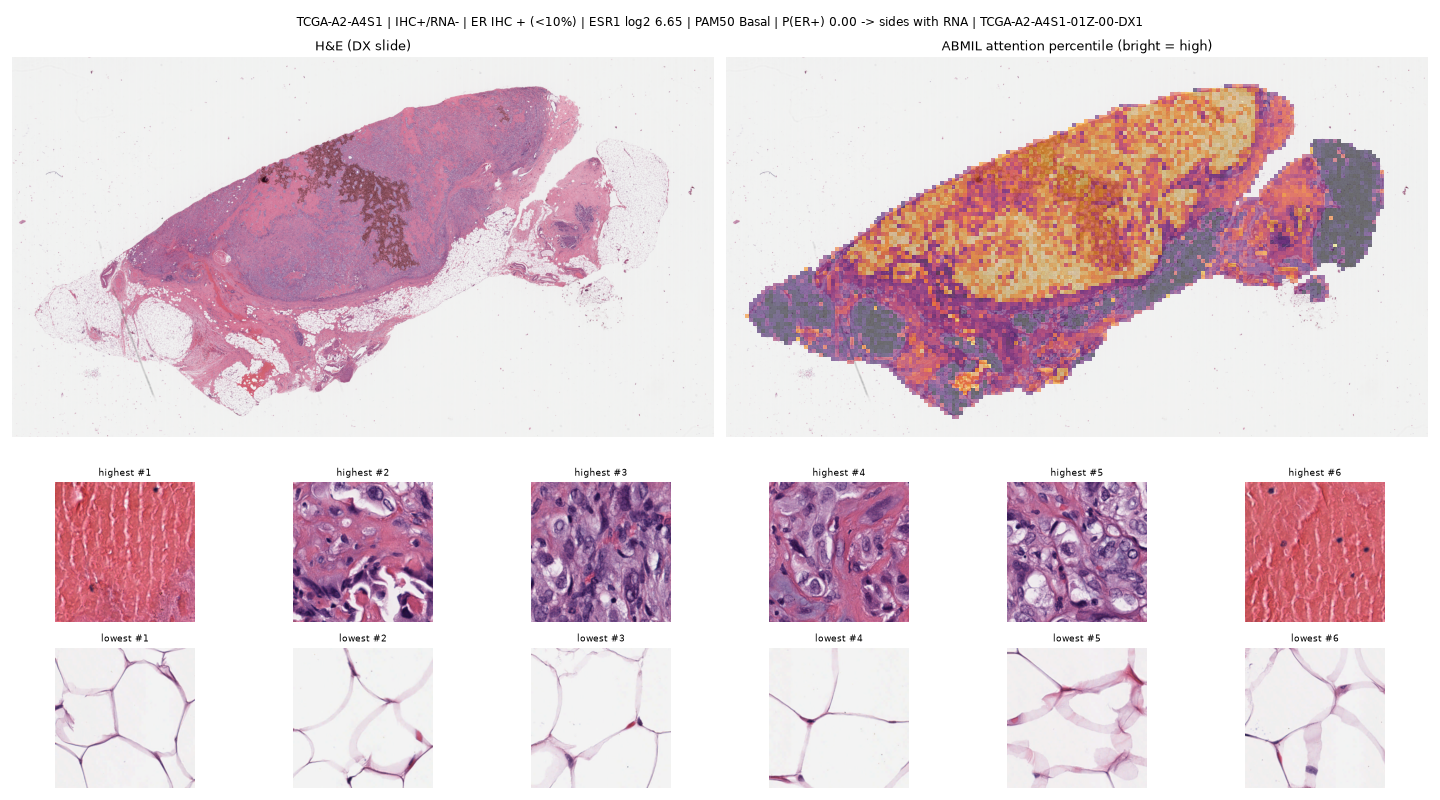
\includegraphics[width=\linewidth]{../results/attention_overlay/TCGA-A2-A4S1.png}\\[-1pt]
{\tiny ER-low (IHC+, $<$10\%), RNA$-$, Basal $\rightarrow$ called ER$-$ (with RNA)}
\end{column}
\begin{column}{0.49\textwidth}
\centering
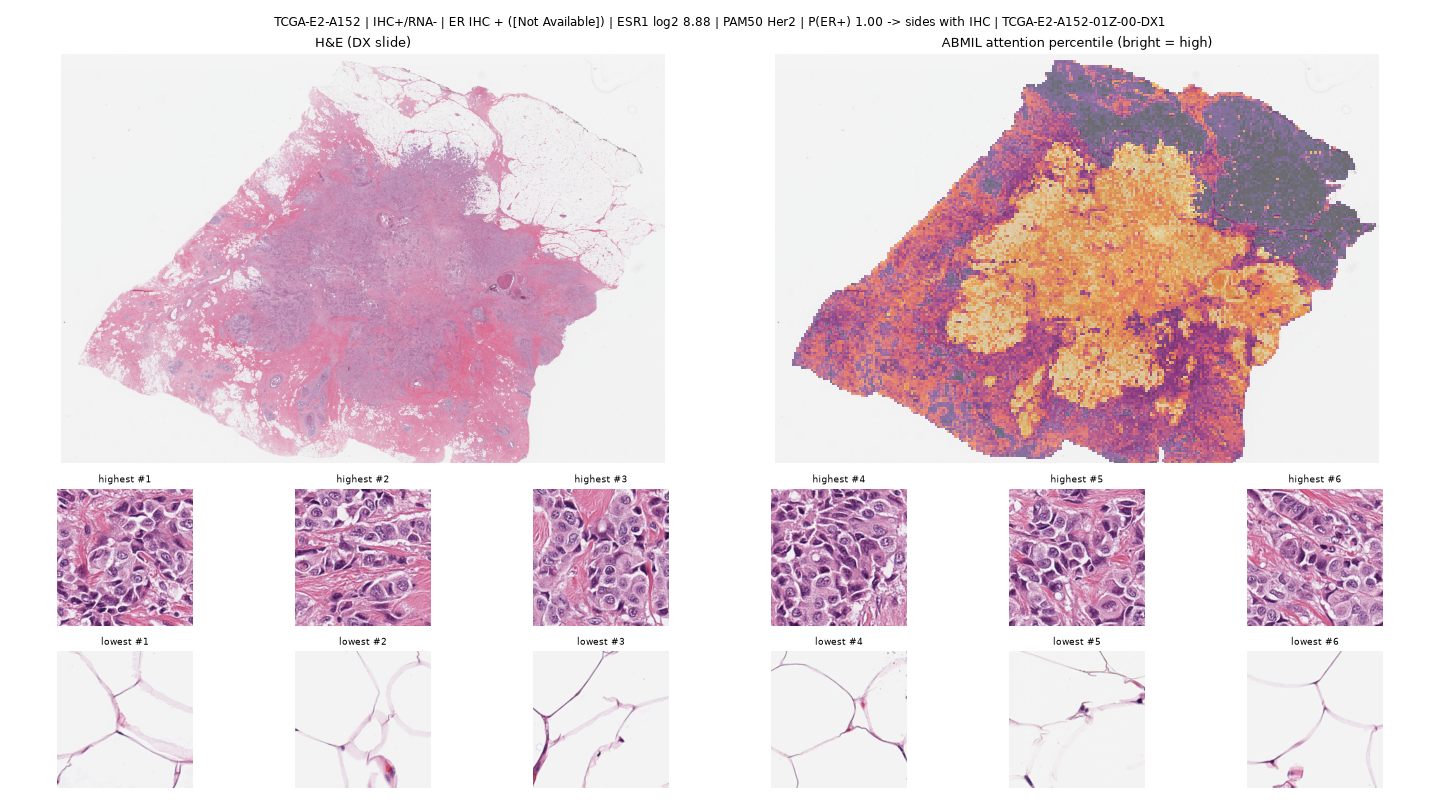
\includegraphics[width=\linewidth]{../results/attention_overlay/TCGA-E2-A152.png}\\[-1pt]
{\tiny IHC+, RNA$-$, HER2-enriched $\rightarrow$ called ER+ (with IHC)}
\end{column}
\end{columns}
\vspace{4pt}
\begin{itemize}
  \item 10 patients, slides from the IDC copy; top/bottom rows = 6 highest / lowest attention patches at 20$\times$.
  \item \textbf{Attention sits on tumour} in every slide reviewed; fat, glass and ink get the least.
  \item ER-low Basal tumours look like the ER$-$ reference (high-grade, pleomorphic) $\rightarrow$ called ER$-$.
  \item HER2-enriched exceptions: attention on cohesive / apocrine-like cells $\rightarrow$ called ER+ (to confirm with a pathologist).
  \item Caveat: some attention on blood or stroma; six slides illustrate, they do not test.
\end{itemize}
\end{frame}

%===================================================================
\begin{frame}[t]{Frozen slides: 1c (FFPE vs frozen) and 1e (two frozen sections)}
\footnotesize
\textbf{Data:} 1,515 frozen slides (1,044 top TS, 471 bottom BS) from the IDC copy, TRIDENT + UNI v1 at 20$\times$.
Our pipeline reproduces the TRACE DX features exactly (46 slides, cosine 1.0000), so DX vs TS differ only in tissue.
\vspace{3pt}

\centering
\scriptsize
\begin{tabular}{lrcccc}
\toprule
\textbf{1c} (same patients, same folds) & $n$ & DX $\Delta$AUC & TS $\Delta$AUC & Interaction (95\% CI) & $p$ \\
\midrule
\textbf{ER: RNA $-$ IHC} & 947 & +0.032 & +0.032 & \textbf{0.000} ($-$0.024, +0.024) & 0.98 \\
ER: RPPA $-$ IHC & 777 & +0.041 & +0.007 & $-$0.035 ($-$0.066, $-$0.001) & 0.045 \\
PR: RNA $-$ IHC (prev.-matched) & 944 & $-$0.003 & +0.026 & +0.029 ($-$0.007, +0.066) & 0.12 \\
HER2: amplif. $-$ strict & 537 & +0.045 & +0.014 & $-$0.030 ($-$0.110, +0.046) & 0.44 \\
\bottomrule
\end{tabular}

\vspace{4pt}
\begin{tabular}{lrcccc}
\toprule
\textbf{1e} (373 TS+BS pairs) & pairs & ICC (logit P) & Cohen's $\kappa$ & calls flipped & AUC TS / BS \\
\midrule
ER model, IHC label & 368 & 0.871 & 0.725 & 10.9\% & 0.891 / 0.877 \\
ER model, RNA label & 367 & 0.892 & 0.806 & 7.6\% & 0.939 / 0.940 \\
\bottomrule
\end{tabular}

\vspace{4pt}
\raggedright
\begin{columns}[T]
\begin{column}{0.49\textwidth}
\begin{block}{1c: the answer does not change}
The frozen slide cut next to the sequenced tissue prefers RNA over IHC \textbf{exactly as much} as the FFPE slide;
on ER-discordant patients it sides with RNA 39\,:\,13 ($p$ = 0.0004). Not a tissue-sampling artefact.
\end{block}
\end{column}
\begin{column}{0.49\textwidth}
\begin{alertblock}{1e: one slide is not the tumour}
Two sections agree well (ICC $\approx$ 0.88) but \textbf{1 in 10 ER calls flips}; the RNA-trained model is somewhat
more reproducible.
\end{alertblock}
\end{column}
\end{columns}
\end{frame}

%===================================================================
\begin{frame}[t]{Plan for the next week}
\footnotesize
\begin{columns}[T]
\begin{column}{0.32\textwidth}
\begin{block}{Done this week}
\begin{itemize}
  \item Final tables for 1a--1e (fixed splits, one environment).
  \item Primary vs secondary claims; multiple-testing note.
  \item Sanity checks S1--S15 incl.\ frozen slides.
\end{itemize}
\end{block}
\end{column}
\begin{column}{0.32\textwidth}
\begin{block}{Next}
\begin{itemize}
  \item External check on CPTAC-BRCA (IDC slides; 1a/1b).
  \item Final report and presentation.
\end{itemize}
\end{block}
\end{column}
\begin{column}{0.32\textwidth}
\begin{block}{Interpretation \& write-up}
\begin{itemize}
  \item Heatmaps on slide thumbnails (does attention sit on tumour?).
  \item HER2-enriched exception.
  \item Final tables + multiple-testing note.
\end{itemize}
\end{block}
\end{column}
\end{columns}

\vspace{10pt}
\centering
\begin{tabular}{lr}
\toprule
Primary claims & Status \\
\midrule
ER: RNA label more predictable than IHC (1a) & supported (Holm-adj.\ p = 0.042; 4 of 5 variants) \\
ER: model sides with RNA on discordant cases (1b) & suggestive (Holm-adj.\ p = 0.15); frozen 39\,:\,13 \\
ER: same answer on FFPE and frozen slides (1c) & interaction 0.000 ($-$0.024, +0.024) \\
HER2 tracks amplification (1b) & p = 0.003 (1a encoder-dependent) \\
PR: no preference; HER2-low invisible & robust nulls \\
\bottomrule
\end{tabular}
\end{frame}

\end{document}
